%%%%%%%%%%%%%%%%%%%%%%%%%%%%%%%%%%%%%%%%%%%%%%%%%%%%%%%%%%%%%
%
%%  LAB4 : Face Detection
%%  Fabrizio Pedersoli 72816
%%  Mohmad Farran 73606
%  
%%%%%%%%%%%%%%%%%%%%%%%%%%%%%%%%%%%%%%%%%%%%%%%%%%%%%%%%%%%%%
\documentclass[a4paper,11pt]{article}

\usepackage[italian]{babel}
\usepackage[utf8]{inputenc}
\usepackage[T1]{fontenc}
\usepackage[a4paper,margin=3.5cm]{geometry}
%\usepackage[scaled]{helvet} 
\usepackage{palatino,euler}
\usepackage{graphicx,subfigure,psfrag}
\usepackage{hyperref}
\usepackage{pdfsync}
\usepackage{amsmath,amssymb,amsfonts,amstext}
\usepackage{siunitx}
%\usepackage{booktabs,multirow}
\usepackage[table]{xcolor}
%\usepackage{supertabular}

\usepackage{listings} 
\lstset{basicstyle=\footnotesize, frame=single,%
  language=C,linewidth=0.8\linewidth}
  

\newcommand{\cv}{OpenCV}

%============================================================
\begin{document}

%%

\begin{titlepage} 
 
\begin{center}
  
  {\bfseries \scshape \Large UNIVERSIT\'A DEGLI STUDI DI BRESCIA
    \\[0.2cm] 
    FACOLT\'A DI INGEGNERIA}\\ [0.35cm]

  {CORSO DI LAUREA SPECIALISTICA IN INGEGNERIA DELLE TELECOMUNICAZIONI}\\ [0.7cm]
  
  {\Large \emph{Laboratorio specialistico Campi/TLC}}\\[10mm]

  \begin{figure}[!h]
    \centering
    
\includegraphics[scale=0.7]{logo}
  \end{figure}
     
  \vspace{1cm}

  {\huge\bfseries Face Detection}\\[0.2cm]

  \vspace{2cm}
  
  \begin{flushleft} \large
    Studenti: \\
    \textbf{Mohamad Farran} \hfill Matricola: \textbf{73606}\\
    \textbf{Fabrizio Pedersoli} \hfill Matricola: \textbf{72816}
\end{flushleft}
 
\vfill

{\large ANNO ACCADEMICO 2009/2010}
    
\end{center}

\end{titlepage}


%%% Local Variables: 
%%% mode: latex
%%% TeX-master: "main"
%%% End: 

\tableofcontents

%------------------------------------------------------------
\section{Introduzione}
\label{sec:intro}
Quest'esperienza di laboratorio si focalizza su di un particolare ed
importante algoritmo implementato all'interno delle Open Source
Computer Vision Library (\cv{}).

\cv{} sono delle librerie open-source sviluppate da Intel, scritte in
C e progettate per ottenere un'elevata efficienza computazionale con
particolare interesse alle applicazione real-time. Queste forniscono
all'utente una semplice interfaccia attraverso cui, con poco sforzo, è
possibile realizzare sofisticate applicazioni di computer vision.

Con computer vision si intende il processo di trasformazione dei dati
rappresentativi di un'immagine od un video in una ``decisione'' oppure
in un nuovo tipo di rappresentazione. L'algoritmo studiato in questa
esperienza è un esempio fondamentale, nonché di grande interesse, di
questo tipo di applicazioni. L'algoritmo di Viola-Jones permette
infatti il riconoscimento dei volti all'interno di un'immagine
(face-detection).

%------------------------------------------------------------
\section{Face Detection}
\label{sec:face}
\cv{} fornisce un face-detector pronto all'uso chiamato Haar
Classifier. 

Data un'immagine od un flusso video, il face-detector esamina ogni
posizione e classifica la rispettiva zona in ``face'' o
``non-face''. Siccome un'immagine può raffigurare volti di dimensioni
differenti, l'algoritmo deve essere eseguito svariate volte
utilizzando scale diverse (default $50\times 50$ pixel), esso presenta
delle ottimizzazione che rendono molto efficienti (descritte in
sec.~\ref{sec:vj}) tutte queste operazioni che sembrano richiedere
un'elevato carico computazionale.

Il classificatore utilizza dei dati archiviati in appositi file XML
per poter classificare una data porzione di immagine. \cv{} fornisce
diversi file adatti per contesti diversi, in particolare è presente un
file per il face-detection ``frontale'' oppure per il profilo, e non
solo: include anche un non-face file e full, upper, lower body.

\subsection{Viola-Jones}
\label{sec:vj}
Il face-detector implementato nelle \cv{} utilizza il metodo
sviluppato da Paul Viola e Micheal Jones pubblicato nel 2001 dal
titolo ``Rapid Object Detection using a Boosted Cascade of Simple
Features''. Quest'approccio combina principalmente quattro fattori
chiave:

\begin{itemize}
\item Semplici features rettangolari definite Haar features
\item L'immagine integrale per velocizzare la classificazione
\item Il metodo AdaBoost
\item Un classificatore in cascata per combinare efficientemente i
  risultati
\end{itemize}

Il metodo Viola-Jones utilizza per la classificazione delle features
denominate ``Haarlike'' del tipo mostrato in fig.~\ref{fig:haarlike}.

\begin{figure}[htbp]
  \centering
  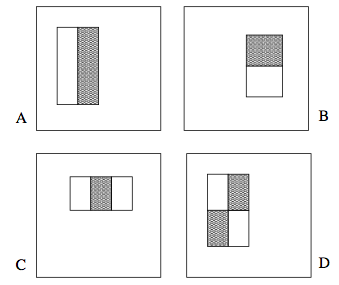
\includegraphics[scale=0.5]{haarlike}
   \caption{Haarlike features}
  \label{fig:haarlike}
\end{figure}

La presenza di una Haar feature è determinata dalla sottrazione del
valor medio dei pixel nella regione scura con il valor medio nella
regione chiara. Se la differenza supera una certa soglia impostata
durante la fase di training, allora tale features è presente. Per
rendere più veloce la procedura di individuazione delle Haar features
il metodo Viola-Jones propone l'utilizzo dell'immagine integrale,
definita come:

\[
ii(x,y) = \sum_{\substack{x^{'}\leq\,x\\ y'\leq\, y}} i(x^{'},y^{'})
\]

per mezzo dell'immagine integrale risulta molto veloce il calcolo
dell'integrale in un qualsiasi rettangolo arbitrario, ad esempio in
fig.~\ref{fig:int}

\begin{figure}[htbp]
  \centering
  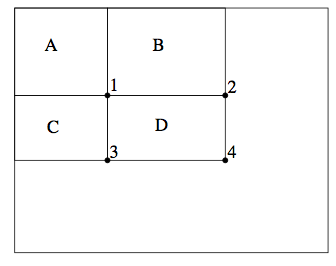
\includegraphics[scale=0.5]{int}
  \caption{int}
  \label{fig:int}
\end{figure}

\[ 
D = A+B+C+D - (A+B) - (A+C) +A 
\]

quindi per calcolare D viene effettuata solamente una semplice
operazione tra interi:

\[
D = (x_{4},y_{4}) - (x_{2},y_{2}) - (x_{3}, y_{3}) + (x_{1}, y_{1})
\]

Per selezionare l'Haar feature da utilizzare ed il relativo valore si
soglia questo algoritmo adopera il metodo AdaBoost. 

AdaBoost crea un classificatore ``forte'' utilizzando tanti
classificatori ``deboli'' . Viola-Jones combina le classificazioni
deboli in una catena di filtri del tipo in fig.~\ref{fig:filtri}

\begin{figure}[htbp]
  \centering
  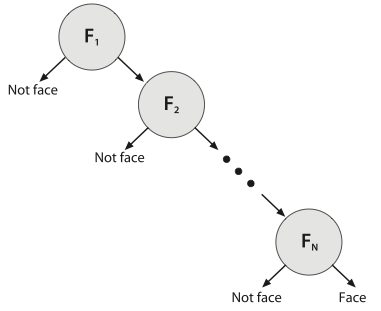
\includegraphics[scale=0.5]{filtri}
  \caption{filtri}
  \label{fig:filtri}
\end{figure}

al fine di ottenere una classificazione efficiente. In pratica ogni
filtro è un classificatore debole che rappresenta un Haar feature con
un valore di soglia settato in modo tale da dare un risposta positiva
per ogni immagine di training. Una regione è classificata ``face'' se
passa tutta la catena di filtri. L'ordinamento dei filtri non è
casuale ma è determinato dai pesi assegnati tramite AdaBoost, in
pratica i filtri con più ``peso'' si trovano nelle prime posizioni
così che le regioni ``non-face'' siano scartate il più velocemente
possibile.

%------------------------------------------------------------
\section{Analisi dell'implementazione in \cv{}}
\label{sec:imp}
Come è stato visto precedentemente \cv{} offre un object-detector
basato sul metodo viola-jones. 

Come prima cosa però è necessario effettuare una fase di training, per
cui si lascia agire il classificatore su di un database di qualche
centinaio di oggetti di interesse. Questi oggetti di interesse possono
essere di qualsiasi tipo: volti, auto, \ldots{} una volta effettuato il
training il metodo funziona indistintamente dal tipo di oggetto da
rilevare. Questo procedimento, nel caso di volti, lo esegue
direttamente \cv{} fornendo degli appositi file XML.

Un volta che il classificatore è stato addestrato viene applicato alla
regione di interesse nell'immagine test, esso restuisce ``1'' o ``0''
a seconda che la regione raffiguri o meno l'oggetto desiderato. A
questo punto non resta altro che far scorrere la finestra di ricerca
in ogni posizione dell'immagine ed eseguire il classificatore. Per
essere in grado di rilevare oggetti a dimensioni differenti, il
classificatore è stato progettato in modo da essere ridimensionato di
conseguenza, così che sia più efficiente rispetto a ridimensionare
l'immagine test. Pertanto per trovare un oggetto di dimensione
incognita l'intera procedura di classificazione deve essere eseguita
svariate volte a scale differenti.

Si ricorda inoltre che il classificatore è costituito da un cascata
(cascade) di classificatori più semplici (stages), bastati sulle
Haarlike feature ed applicati sequenzialmente alla regione di
interesse, al primo stage che fallisce la procedura viene interrotta
restituendo ``0'' (oggetto non trovato). La catena di classificatori è
progettata tramite il metodo AdaBoost, in modo da posizionare nelle
prime posizioni quelli più significativi.

%------------------------------------------------------------
\subsection{Boosted cascade classifier}
\label{sec:class}
Di seguito saranno descritte le strutture che implementano il
classificatore delle \cv{}

\subsubsection{CvHaarFeature}
\label{sec:cvhaarfeatyre}

\begin{lstlisting}
#define CV_HAAR_FEATURE_MAX 3

typedef struct CvHaarFeature
{
  int titled;
  struct
  {
    CvRect r;
    float weight;
    rect[CV_HAAR_FEATURE_MAX];
  }
} CvHaarFeature;
\end{lstlisting}

definisce una haar feature, orizzontale/verticale oppure ruotata di
\ang{45}, a seconda del valore di \emph{titled}, che consiste in 2-3
rettangoli con il relativo penso.

\subsubsection{CvHaarClassifier}
\label{sec:cvhaarclassifier}

\begin{lstlisting}
typedef struct CvHaarClassifier
{
  int count;
  CvHaarFeature* haar_feature;
  float* threshold;
  int* left;
  int* right;
  float* alpha;
}  
CvHaarClassifier;
\end{lstlisting}

un singolo albero di classificazione, valutato
in una particolare posizione dell'immagine test, che riporta il
risultato delle haar feature testate nei rispettivi rami (\emph{left}
e \emph{right}).

\subsubsection{CvHaarStageClassifier}
\label{sec:cvhaarstageclassifier}

\begin{lstlisting}
typedef struct CvHaarStageClassifier
{
  int count;
  float threshold;
  CvHaarClassifier* classifier;
  int next;
  int child;
  int parent;
} 
CvHaarStageClassifier;
\end{lstlisting}

costituisce il classificatore stage: continente un'array di
cvHaarClassifier ed il valore di soglia a livello di stage.

\subsubsection{CvHaarClassifierCascade}
\label{sec:cvhaarclassifiercascade}

\begin{lstlisting}
typedef struct CvHaarClassifierCascade
{
  int flags;
  int count;
  CvSize orig_window_size;
  CvSize real_window_size;
  double scale;
  CvHaarStageClassifier* stage_classifier;
  CvHidHaarClassifierCascade* hid_cascade;
} 
CvHaarClassifierCascade;
\end{lstlisting}

cascata dei classificatori stage, definisce parametri quali: le
dimensioni delle finestra di ricerca, il fattore di scale ed una
versione ottimizzata del cascade.


%------------------------------------------------------------
\subsection{Funzioni per l' object detection}
\label{sec:detect}
In questa sottosezione si vedranno le principali funzioni costituenti
l'object-detector

\subsubsection{cvHaarDetectObjects}
\label{sec:cvhaar}

\begin{lstlisting}
  CvSeq* 
  cvHaarDetectObjects(
          const CvArr* image,
          CvHaarClassifierCascade* cascade,
          CvMemStorage* storage,
          double scale_factor=1.1,
          int min_neighbors=3,
          int flags=0,
          CvSize min_size(0,0))
\end{lstlisting}

richiede come parametri 

\begin{itemize}
\item \emph{image } immagine test.
\item \emph{cascade} Haar classifier cascade
\item \emph{storage} area di memoria utilizzata per immagazzinare la
  sequenza di rettangoli candidati a contenere l'oggetto di interesse
\item \emph{scale\_factor} fattore di scala attraverso cui la finestra
  di ricerca viene riscalata nelle scansioni successive
\item \emph{min\_neighbors} numero minimo di rettangoli ``vicini'' che
  creano un'oggetto. Se questo parametro viene settato a zero, non
  viene effettuato alcun raggruppamento, per cui la funzione
  restituirà tutti i rettangoli candidati.
\item \emph{flags} un flag che indica la modalità di funzionamento,
  praticamente l'unico che può essere specificato, \texttt{\small
    CV\_HAAR\_DO\_CANNY\_PRUNING}. Se questo è settato la funziona
  utilizza un Canny edge detector per rifiutare particolari regioni
  che contengono troppi, o troppo pochi edge, e che pertanto si
  ritiene che non conterraneo l'oggetto ricercato.
\item il valore minimo delle finestra di ricerca, di default
  coincide che le dimensioni dei campioni utilizzati durante il
  training.
\end{itemize}

Questa è la funzione principale, trova le regioni rettangolari
nell'immagine test che soddisfano il classificatore, e ritorna tali
zone come una sequenza di rettangoli. Questa funzione scansiona
l'immagine diverse volte a differenti scale, ogni volta considera
regioni sovrapposte ed esegue il classificatore attraverso la funzione
\emph{RunHaarClassifierCascade}. Può applicare inoltre qualche
euristica, tipo il Canny pruning, al fine di ridurre le regioni da
analizzare velocizzando la scansione.


\subsubsection{cvSetImageForHaarClassifierCascade}
\label{sec:setimage}

\begin{lstlisting}
  void  
  cvSetImagesForHaarClassifierCascade(
            CvHaarClassifierCascade* cascade, 
            const Cvarr* sum, 
            const CvArr* sqsum, 
            const CvArr titled_sum, 
            double scale)
\end{lstlisting}

richiede come parametri:

\begin{itemize}
\item \emph{cascade} Haar classifier cascade 
\item \emph{sum} immagine integrale a singolo canale a 32bit
\item \emph{sqsum} immagine intergrale degli elementi al quadrato in
  formato 64bit floating point
\item \emph{scale} fattore di scale per la finestra di ricerca
\end{itemize}

Questa funzione è utilizzata per preparare il cascade per il
riconoscimento di oggetti di una particolare dimensione nell'immagine
test.

\subsubsection{RunHaarClassifierCascade}
\label{sec:run}

\begin{lstlisting}
  int
  cvRunHaarClassifierCascade(
         CvHaarClassifierCascade* cascade,
         CvPoint pt, 
         int start_stage=0)
\end{lstlisting}

richiede come parametri:

\begin{itemize}
\item \emph{cascade} Haar classifier cascade
\item \emph{pt} angoli sinistro superiore della regione da analizzare
\item \emph{start\_stage} indica l'indice della cascata da cui partire
\end{itemize}

Questa funzione esegue il classificatore cascade in una singola
posizione nell'immagine test. Prima di utilizzare tale funzione è
necessario aver settato l'immagine integrale e l'appropriata
dimensione delle finestra di ricerca attraverso la funzione
\emph{SetImageForHaarClassifierCascade}. Viene ritornato un valore
positivo se il rettangolo analizzato soddisfa l'intera cascata, zero
od un valore negativo altrimenti.


%------------------------------------------------------------
\section{Simulazioni}
\label{sec:simulazioni}
In questa sezione saranno commentati i risultati di face-detecion su
di un'immagine test, di dimensione $640\times480$, al variare dei
principali parametri della funzione
\emph{cvHaarDetectObjects}. Operativamente si andrà ad agire su
\emph{min\_neighbors}, \emph{flags} e \emph{min\_size}.

Il parametro \emph{min\_neighbors}, fig.~\ref{fig:minneigh}, è
fondamentale affinché non ci siano falsi riconoscimenti, infatti una
zona in cui è presente una faccia tende solitamente a riportare
riconoscimenti multipli. Settare questo parametro per esempio a 3
significa che viene riconosciuto un volto qualora ci siano almeno 3
regioni sovrapposte classificate come tale.

\begin{figure}[htbp]
  \centering
  \subfigure[1]%
  {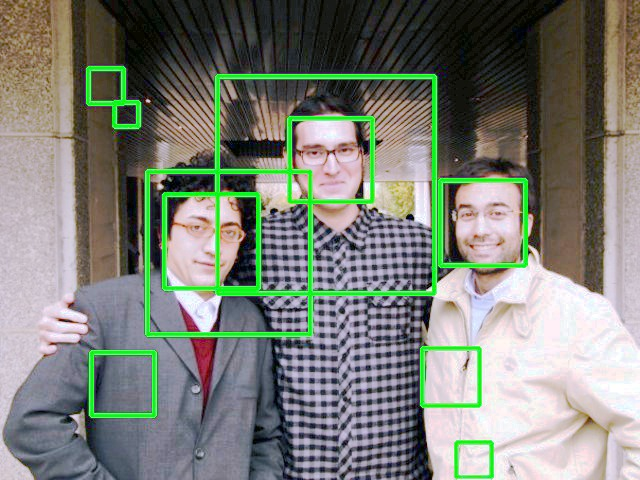
\includegraphics[scale=0.28]{../code/min1}\label{fig:min1}}
  \hspace{2mm}
  \subfigure[3]%
  {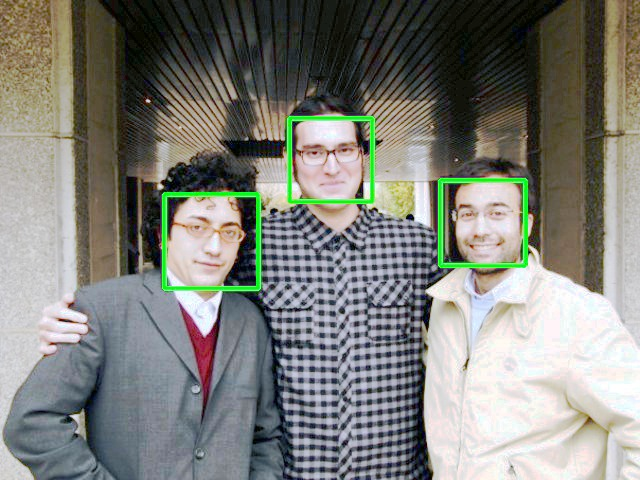
\includegraphics[scale=0.28]{../code/min3}\label{fig:min2}}
  \caption{risultati al variare di \emph{min\_neighbors}}
  \label{fig:minneigh}
\end{figure}

si noti come nel caso fig.~\ref{fig:min1} siano presenti delle false
classificazioni, mentre in fig.~\ref{fig:min2} i volti vengono
rilevati correttamente.\\

Modificano invece il valore di \emph{min\_size},
fig.~\ref{fig:minsize} si indica il la dimensione minima della
finestra di ricerca. Il valore di default coincide con la dimensione
utilizzata in fase di training, che è specificata nel file XML
utilizzato. La variazione di questo parametro permette di velocizzare
la ricerca, anche di molto, se si ha un conoscenza a priori della
dimensione delle facce da ricercare.

\begin{figure}[htbp]
  \centering
  \subfigure[100]%
  {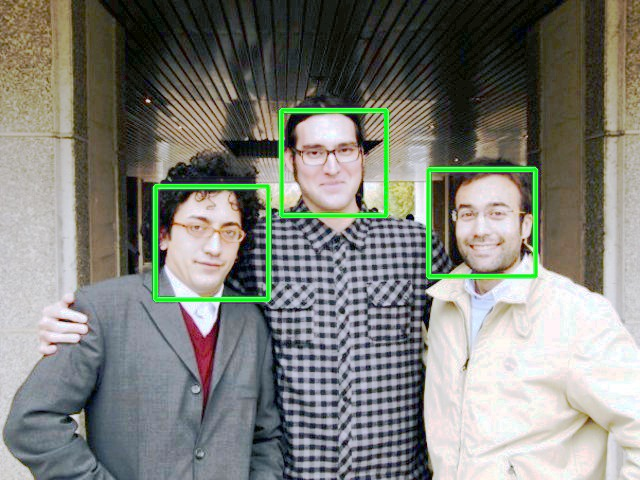
\includegraphics[scale=0.28]{../code/size100}\label{fig:s100}}
  \subfigure[110]%
  {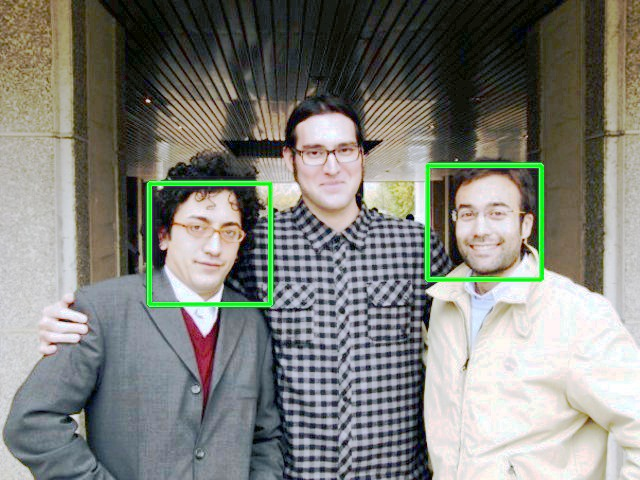
\includegraphics[scale=0.28]{../code/size110}\label{fig:s110}}
  \subfigure[120]%
  {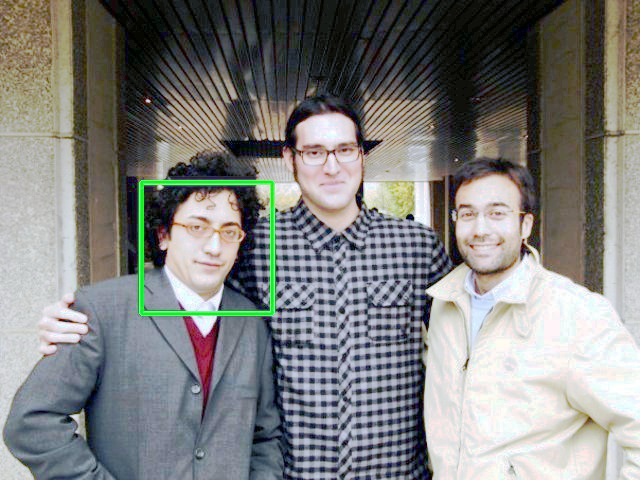
\includegraphics[scale=0.28]{../code/size120}\label{fig:s120}}
  \subfigure[150]%
  {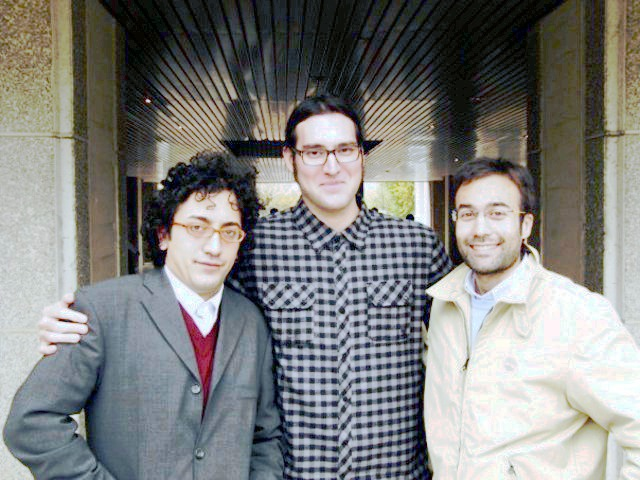
\includegraphics[scale=0.28]{../code/size150}\label{fig:s150}}
  \caption{risultati al variare di \emph{min\_size}}
  \label{fig:minsize}
\end{figure}

Si noti come in questo caso utilizzando una dimensione minima della
finestra di $150$, fig.~\ref{fig:s150}, non si ha riconoscimento, con
$120$, fig.~\ref{fig:s120}, si ha un riconoscimento parziale (una su
tre) con $110$, fig.~\ref{fig:s110}, (due su tre), con $100$,
fig.~\ref{fig:s100}, si ha un riconoscimento totale.\\

Attraverso il parametro \emph{flags} si modifica in modo marginale il
comportamento della funzione. Operativamente con \texttt{\small
  CV\_HAAR\_SCALE\_IMAGE} si indica all'algoritmo di scalare
l'immagine piuttosto che il classificatore, mentre con \\
\texttt{\small CV\_HAAR\_FIND\_BIGGEST\_OBJECT} si fa si che la
funzione ritorni solamente l'oggetto più grosso tra quelli trovati,
fig.~\ref{fig:minsize}.

\begin{figure}[htbp]
  \centering
  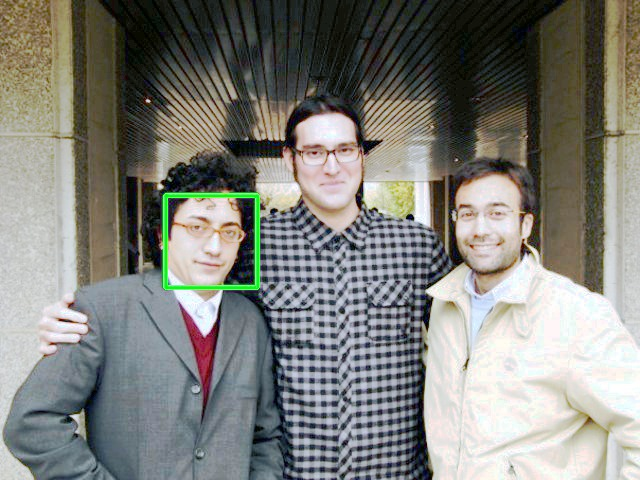
\includegraphics[scale=0.28]{../code/big}
  \caption{rilevazione dell'oggetto più grande}
  \label{fig:big}
\end{figure}



%============================================================
\end{document}
